\documentclass{article}
\usepackage{tikz}
\usetikzlibrary{positioning, shapes.geometric}

\begin{document}

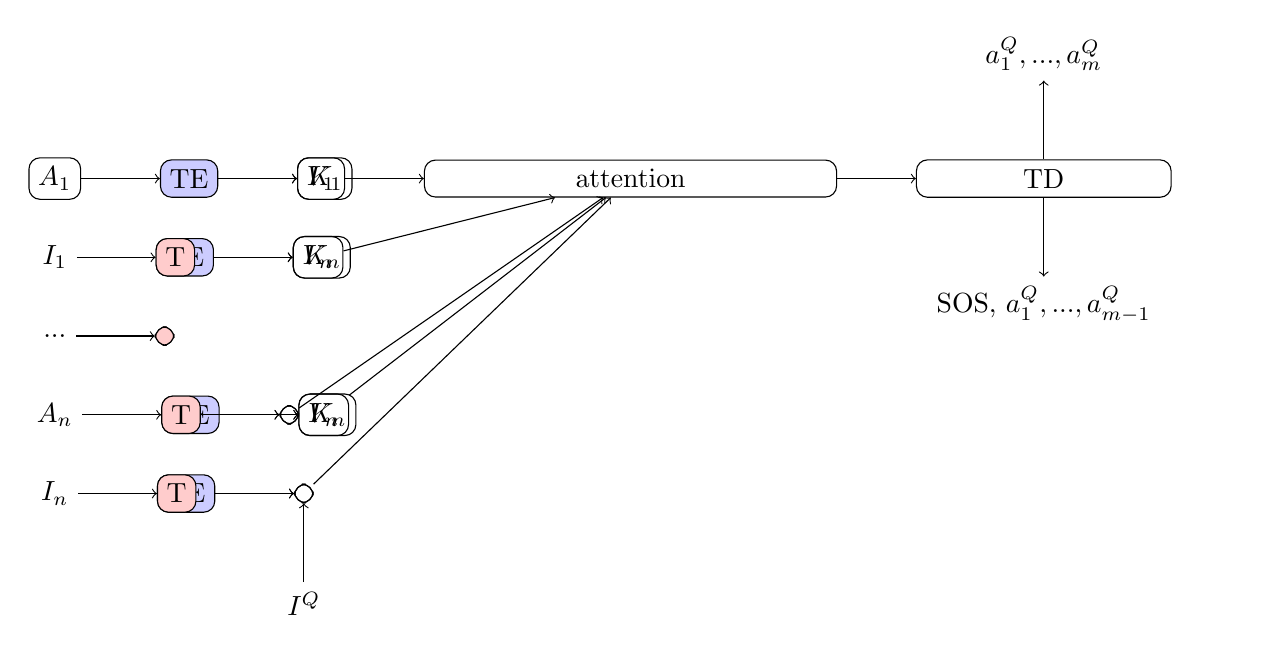
\begin{tikzpicture}[node distance=1cm, auto]
    \node (input) [draw, rounded corners] {$A_{1}$};
    \node (input2) [below of=input] {$I_{1}$};
    \node (input3) [below of=input2] {...};
    \node (input4) [below of=input3] {$A_{n}$};
    \node (input5) [below of=input4] {$I_{n}$};

    \node (te1) [draw, rounded corners, right=of input, fill=blue!20] {TE};
    \node (te2) [draw, rounded corners, right=of input2, fill=blue!20] {TE};
    \node (te3) [draw, rounded corners, right=of input3, fill=blue!20] {};
    \node (te4) [draw, rounded corners, right=of input4, fill=blue!20] {TE};
    \node (te5) [draw, rounded corners, right=of input5, fill=blue!20] {TE};

    \node (t1) [draw, rounded corners, right=of input2, fill=red!20] {T};
    \node (t2) [draw, rounded corners, right=of input3, fill=red!20] {};
    \node (t3) [draw, rounded corners, right=of input4, fill=red!20] {T};
    \node (t4) [draw, rounded corners, right=of input5, fill=red!20] {T};

    \node (v1) [right=of te1, draw, rounded corners] {$V_{1}$};
    \node (v2) [right=of te2, draw, rounded corners] {$V_{n}$};
    \node (v3) [right=of t3, draw, rounded corners] {};
    \node (v4) [right=of te4, draw, rounded corners] {$V_{n}$};
    \node (v5) [right=of te5, draw, rounded corners] {};

    \node (k1) [right=of te1, draw, rounded corners] {$K_{1}$};
    \node (k2) [right=of te2, draw, rounded corners] {$K_{n}$};
    \node (k3) [right=of t3, draw, rounded corners] {};
    \node (k4) [right=of te4, draw, rounded corners] {$K_{n}$};
    \node (k5) [right=of te5, draw, rounded corners] {};

    \node (attention) [draw, rounded corners, right=of v1, text width=5cm, align=center] {attention};

    \node (td) [draw, rounded corners, right=of attention, text width=3cm, align=center] {TD};

    \node (output) [above=of td, text width=5cm, align=center] {$a^{Q}_{1}, ..., a^{Q}_{m}$};

    \node (sos) [below=of td, text width=5cm, align=center] {SOS, $a^{Q}_{1}, ..., a^{Q}_{m-1}$};

    \node (iq) [below=of k5, text width=1cm, align=center] {$I^{Q}$};

    \draw[->] (input) -- (te1);
    \draw[->] (input2) -- (t1);
    \draw[->] (input3) -- (t2);
    \draw[->] (input4) -- (te4);
    \draw[->] (input5) -- (te5);

    \draw[->] (te1) -- (v1);
    \draw[->] (te2) -- (v2);
    \draw[->] (t3) -- (v3);
    \draw[->] (te4) -- (v4);
    \draw[->] (te5) -- (v5);

    \draw[->] (te1) -- (k1);
    \draw[->] (te2) -- (k2);
    \draw[->] (t3) -- (k3);
    \draw[->] (te4) -- (k4);
    \draw[->] (te5) -- (k5);

    \draw[->] (v1) -- (attention);
    \draw[->] (v2) -- (attention);
    \draw[->] (v3) -- (attention);
    \draw[->] (v4) -- (attention);
    \draw[->] (v5) -- (attention);

    \draw[->] (attention) -- (td);

    \draw[->] (td) -- (output);
    \draw[->] (td) -- (sos);
    \draw[->] (iq) -- (k5);

\end{tikzpicture}

\end{document}